% Created by tikzDevice version 0.10.1 on 2020-07-01 17:24:47
% !TEX encoding = UTF-8 Unicode
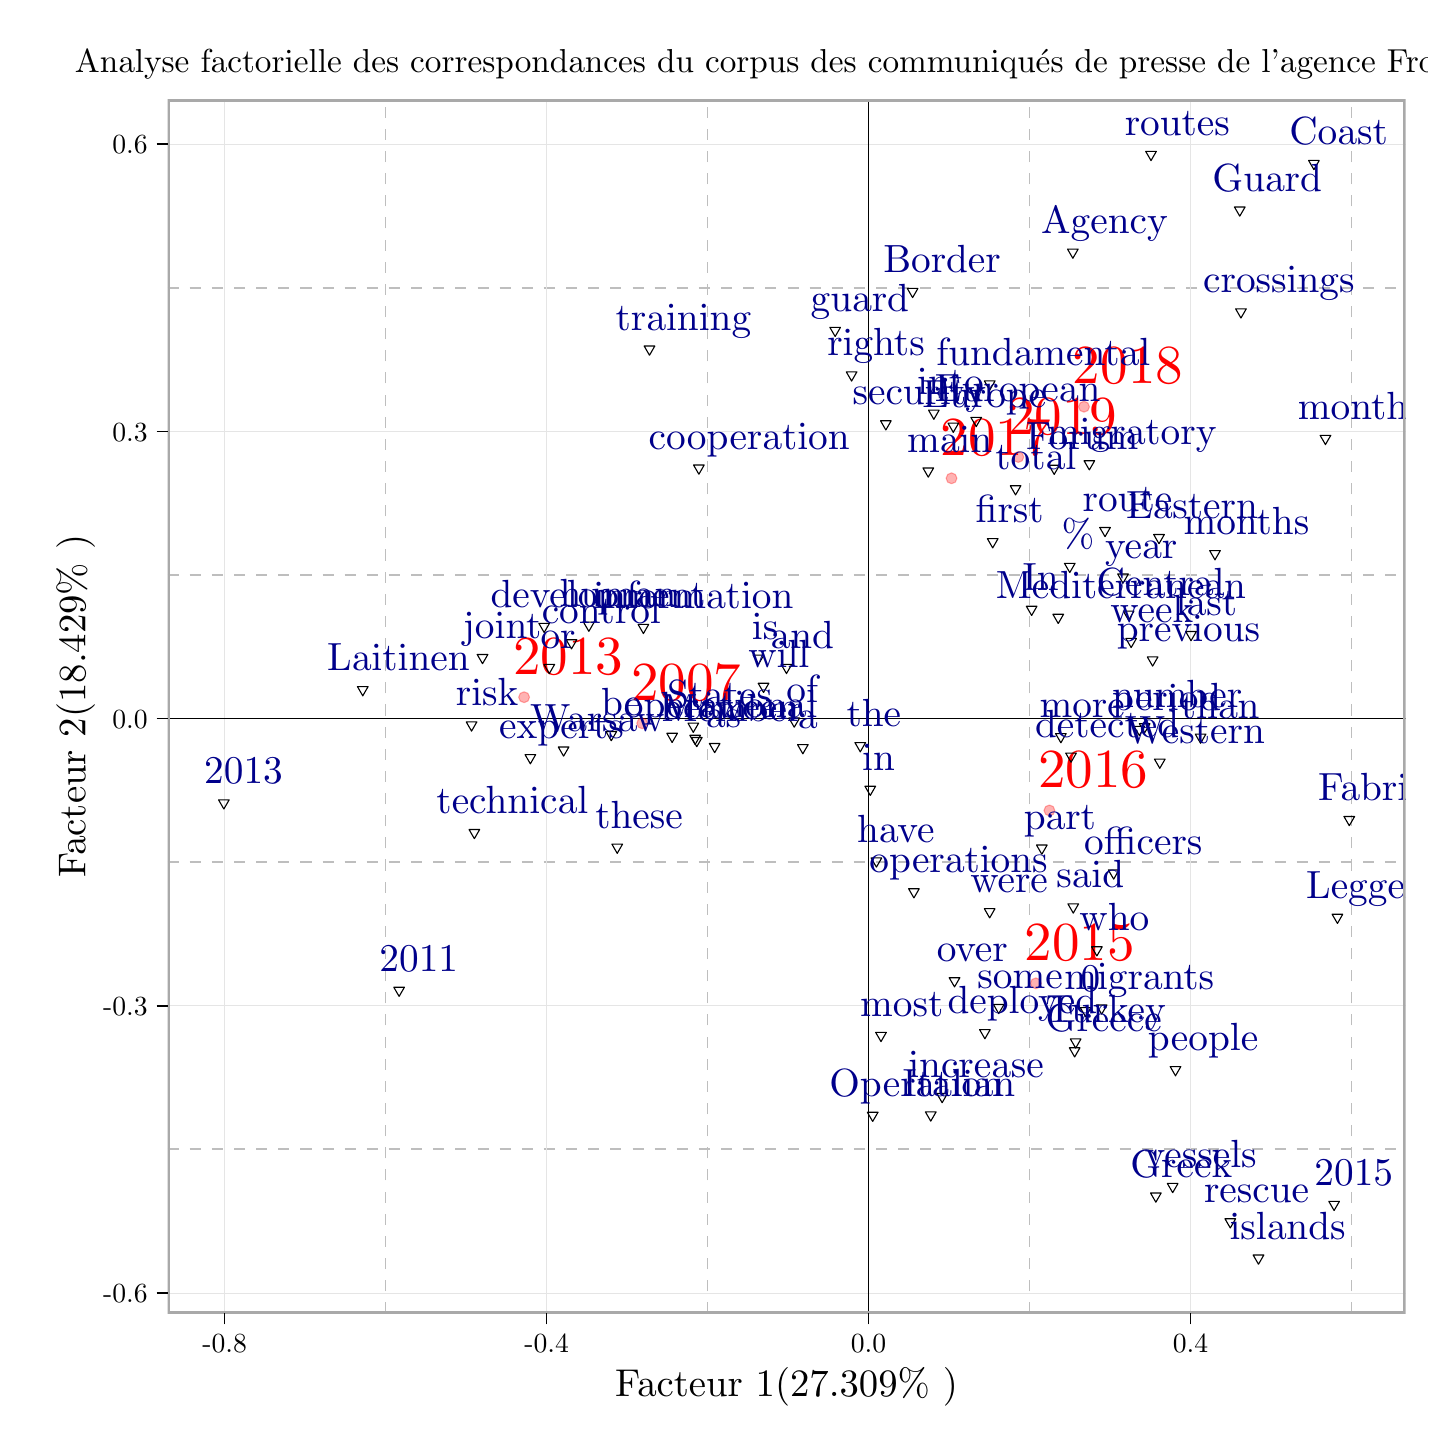
\begin{tikzpicture}[x=1pt,y=1pt]
\definecolor{fillColor}{RGB}{255,255,255}
\path[use as bounding box,fill=fillColor,fill opacity=0.00] (0,0) rectangle (505.89,505.89);
\begin{scope}
\path[clip] (  0.00,  0.00) rectangle (505.89,505.89);
\definecolor{drawColor}{RGB}{255,255,255}
\definecolor{fillColor}{RGB}{255,255,255}

\path[draw=drawColor,line width= 0.6pt,line join=round,line cap=round,fill=fillColor] ( -0.00,  0.00) rectangle (505.89,505.89);
\end{scope}
\begin{scope}
\path[clip] ( 50.56, 41.33) rectangle (497.89,480.02);
\definecolor{fillColor}{RGB}{255,255,255}

\path[fill=fillColor] ( 50.56, 41.33) rectangle (497.89,480.02);
\definecolor{drawColor}{RGB}{190,190,190}

\path[draw=drawColor,line width= 0.6pt,dash pattern=on 4pt off 4pt ,line join=round] ( 50.56,100.60) --
	(497.89,100.60);

\path[draw=drawColor,line width= 0.6pt,dash pattern=on 4pt off 4pt ,line join=round] ( 50.56,204.35) --
	(497.89,204.35);

\path[draw=drawColor,line width= 0.6pt,dash pattern=on 4pt off 4pt ,line join=round] ( 50.56,308.10) --
	(497.89,308.10);

\path[draw=drawColor,line width= 0.6pt,dash pattern=on 4pt off 4pt ,line join=round] ( 50.56,411.85) --
	(497.89,411.85);

\path[draw=drawColor,line width= 0.6pt,dash pattern=on 4pt off 4pt ,line join=round] (129.34, 41.33) --
	(129.34,480.02);

\path[draw=drawColor,line width= 0.6pt,dash pattern=on 4pt off 4pt ,line join=round] (245.68, 41.33) --
	(245.68,480.02);

\path[draw=drawColor,line width= 0.6pt,dash pattern=on 4pt off 4pt ,line join=round] (362.01, 41.33) --
	(362.01,480.02);

\path[draw=drawColor,line width= 0.6pt,dash pattern=on 4pt off 4pt ,line join=round] (478.35, 41.33) --
	(478.35,480.02);
\definecolor{drawColor}{gray}{0.90}

\path[draw=drawColor,line width= 0.2pt,line join=round] ( 50.56, 48.72) --
	(497.89, 48.72);

\path[draw=drawColor,line width= 0.2pt,line join=round] ( 50.56,152.47) --
	(497.89,152.47);

\path[draw=drawColor,line width= 0.2pt,line join=round] ( 50.56,256.22) --
	(497.89,256.22);

\path[draw=drawColor,line width= 0.2pt,line join=round] ( 50.56,359.97) --
	(497.89,359.97);

\path[draw=drawColor,line width= 0.2pt,line join=round] ( 50.56,463.73) --
	(497.89,463.73);

\path[draw=drawColor,line width= 0.2pt,line join=round] ( 71.17, 41.33) --
	( 71.17,480.02);

\path[draw=drawColor,line width= 0.2pt,line join=round] (187.51, 41.33) --
	(187.51,480.02);

\path[draw=drawColor,line width= 0.2pt,line join=round] (303.85, 41.33) --
	(303.85,480.02);

\path[draw=drawColor,line width= 0.2pt,line join=round] (420.18, 41.33) --
	(420.18,480.02);
\definecolor{drawColor}{RGB}{0,0,0}

\path[draw=drawColor,line width= 0.6pt,line join=round] (303.85, 41.33) -- (303.85,480.02);

\path[draw=drawColor,line width= 0.6pt,line join=round] ( 50.56,256.22) -- (497.89,256.22);
\definecolor{drawColor}{RGB}{255,0,0}
\definecolor{fillColor}{RGB}{255,0,0}

\path[draw=drawColor,draw opacity=0.30,line width= 0.4pt,line join=round,line cap=round,fill=fillColor,fill opacity=0.30] (222.06,254.52) circle (  1.96);

\path[draw=drawColor,draw opacity=0.30,line width= 0.4pt,line join=round,line cap=round,fill=fillColor,fill opacity=0.30] (179.38,263.95) circle (  1.96);

\path[draw=drawColor,draw opacity=0.30,line width= 0.4pt,line join=round,line cap=round,fill=fillColor,fill opacity=0.30] (364.30,160.56) circle (  1.96);

\path[draw=drawColor,draw opacity=0.30,line width= 0.4pt,line join=round,line cap=round,fill=fillColor,fill opacity=0.30] (369.20,223.03) circle (  1.96);

\path[draw=drawColor,draw opacity=0.30,line width= 0.4pt,line join=round,line cap=round,fill=fillColor,fill opacity=0.30] (333.83,343.05) circle (  1.96);

\path[draw=drawColor,draw opacity=0.30,line width= 0.4pt,line join=round,line cap=round,fill=fillColor,fill opacity=0.30] (381.70,368.91) circle (  1.96);

\path[draw=drawColor,draw opacity=0.30,line width= 0.4pt,line join=round,line cap=round,fill=fillColor,fill opacity=0.30] (357.96,350.75) circle (  1.96);
\definecolor{drawColor}{RGB}{255,0,0}

\node[text=drawColor,anchor=base west,inner sep=0pt, outer sep=0pt, scale=  1.99] at (218.08,262.75) { 2007};

\node[text=drawColor,anchor=base west,inner sep=0pt, outer sep=0pt, scale=  1.99] at (175.40,272.18) { 2013};

\node[text=drawColor,anchor=base west,inner sep=0pt, outer sep=0pt, scale=  1.99] at (360.31,168.79) { 2015};

\node[text=drawColor,anchor=base west,inner sep=0pt, outer sep=0pt, scale=  1.99] at (365.22,231.27) { 2016};

\node[text=drawColor,anchor=base west,inner sep=0pt, outer sep=0pt, scale=  1.99] at (329.85,351.29) { 2017};

\node[text=drawColor,anchor=base west,inner sep=0pt, outer sep=0pt, scale=  1.99] at (377.72,377.14) { 2018};

\node[text=drawColor,anchor=base west,inner sep=0pt, outer sep=0pt, scale=  1.99] at (353.97,358.99) { 2019};
\definecolor{drawColor}{RGB}{0,0,0}

\path[draw=drawColor,line width= 0.4pt,line join=round,line cap=round] (300.85,244.22) --
	(302.77,247.54) --
	(298.93,247.54) --
	(300.85,244.22);

\path[draw=drawColor,line width= 0.4pt,line join=round,line cap=round] (277.00,253.10) --
	(278.93,256.43) --
	(275.08,256.43) --
	(277.00,253.10);

\path[draw=drawColor,line width= 0.4pt,line join=round,line cap=round] (304.47,228.45) --
	(306.39,231.78) --
	(302.55,231.78) --
	(304.47,228.45);

\path[draw=drawColor,line width= 0.4pt,line join=round,line cap=round] (274.19,272.49) --
	(276.11,275.81) --
	(272.27,275.81) --
	(274.19,272.49);

\path[draw=drawColor,line width= 0.4pt,line join=round,line cap=round] (280.10,243.50) --
	(282.02,246.83) --
	(278.18,246.83) --
	(280.10,243.50);

\path[draw=drawColor,line width= 0.4pt,line join=round,line cap=round] (388.08,149.40) --
	(390.00,152.73) --
	(386.16,152.73) --
	(388.08,149.40);

\path[draw=drawColor,line width= 0.4pt,line join=round,line cap=round] (347.61,184.20) --
	(349.53,187.53) --
	(345.69,187.53) --
	(347.61,184.20);

\path[draw=drawColor,line width= 0.4pt,line join=round,line cap=round] (248.25,243.91) --
	(250.17,247.24) --
	(246.33,247.24) --
	(248.25,243.91);

\path[draw=drawColor,line width= 0.4pt,line join=round,line cap=round] (264.08,275.84) --
	(266.00,279.17) --
	(262.16,279.17) --
	(264.08,275.84);

\path[draw=drawColor,line width= 0.4pt,line join=round,line cap=round] (265.90,265.66) --
	(267.82,268.98) --
	(263.98,268.98) --
	(265.90,265.66);

\path[draw=drawColor,line width= 0.4pt,line join=round,line cap=round] (403.61,251.06) --
	(405.53,254.39) --
	(401.69,254.39) --
	(403.61,251.06);

\path[draw=drawColor,line width= 0.4pt,line join=round,line cap=round] (382.28,148.45) --
	(384.20,151.78) --
	(380.36,151.78) --
	(382.28,148.45);

\path[draw=drawColor,line width= 0.4pt,line join=round,line cap=round] (423.82,247.30) --
	(425.74,250.63) --
	(421.90,250.63) --
	(423.82,247.30);

\path[draw=drawColor,line width= 0.4pt,line join=round,line cap=round] (473.28,182.20) --
	(475.20,185.53) --
	(471.35,185.53) --
	(473.28,182.20);

\path[draw=drawColor,line width= 0.4pt,line join=round,line cap=round] (373.34,247.48) --
	(375.27,250.81) --
	(371.42,250.81) --
	(373.34,247.48);

\path[draw=drawColor,line width= 0.4pt,line join=round,line cap=round] (392.42,198.20) --
	(394.35,201.53) --
	(390.50,201.53) --
	(392.42,198.20);

\path[draw=drawColor,line width= 0.4pt,line join=round,line cap=round] (407.66, 81.47) --
	(409.58, 84.80) --
	(405.74, 84.80) --
	(407.66, 81.47);

\path[draw=drawColor,line width= 0.4pt,line join=round,line cap=round] (414.76,127.15) --
	(416.69,130.48) --
	(412.84,130.48) --
	(414.76,127.15);

\path[draw=drawColor,line width= 0.4pt,line join=round,line cap=round] (378.32,133.95) --
	(380.25,137.28) --
	(376.40,137.28) --
	(378.32,133.95);

\path[draw=drawColor,line width= 0.4pt,line join=round,line cap=round] (306.69,202.54) --
	(308.61,205.87) --
	(304.77,205.87) --
	(306.69,202.54);

\path[draw=drawColor,line width= 0.4pt,line join=round,line cap=round] (342.75,361.74) --
	(344.67,365.07) --
	(340.82,365.07) --
	(342.75,361.74);

\path[draw=drawColor,line width= 0.4pt,line join=round,line cap=round] (366.46,207.20) --
	(368.38,210.53) --
	(364.54,210.53) --
	(366.46,207.20);

\path[draw=drawColor,line width= 0.4pt,line join=round,line cap=round] (377.82,185.94) --
	(379.74,189.26) --
	(375.90,189.26) --
	(377.82,185.94);

\path[draw=drawColor,line width= 0.4pt,line join=round,line cap=round] (395.80,305.14) --
	(397.72,308.47) --
	(393.88,308.47) --
	(395.80,305.14);

\path[draw=drawColor,line width= 0.4pt,line join=round,line cap=round] (386.35,170.45) --
	(388.28,173.78) --
	(384.43,173.78) --
	(386.35,170.45);

\path[draw=drawColor,line width= 0.4pt,line join=round,line cap=round] (320.24,191.42) --
	(322.16,194.74) --
	(318.32,194.74) --
	(320.24,191.42);

\path[draw=drawColor,line width= 0.4pt,line join=round,line cap=round] (477.56,217.52) --
	(479.48,220.84) --
	(475.64,220.84) --
	(477.56,217.52);

\path[draw=drawColor,line width= 0.4pt,line join=round,line cap=round] (210.88,248.22) --
	(212.81,251.55) --
	(208.96,251.55) --
	(210.88,248.22);

\path[draw=drawColor,line width= 0.4pt,line join=round,line cap=round] (413.75, 84.92) --
	(415.67, 88.25) --
	(411.82, 88.25) --
	(413.75, 84.92);

\path[draw=drawColor,line width= 0.4pt,line join=round,line cap=round] (434.56, 72.16) --
	(436.48, 75.48) --
	(432.64, 75.48) --
	(434.56, 72.16);

\path[draw=drawColor,line width= 0.4pt,line join=round,line cap=round] (362.78,293.48) --
	(364.70,296.81) --
	(360.86,296.81) --
	(362.78,293.48);

\path[draw=drawColor,line width= 0.4pt,line join=round,line cap=round] (326.32,110.76) --
	(328.25,114.09) --
	(324.40,114.09) --
	(326.32,110.76);

\path[draw=drawColor,line width= 0.4pt,line join=round,line cap=round] (241.77,246.06) --
	(243.69,249.38) --
	(239.85,249.38) --
	(241.77,246.06);

\path[draw=drawColor,line width= 0.4pt,line join=round,line cap=round] (345.89,140.52) --
	(347.81,143.85) --
	(343.97,143.85) --
	(345.89,140.52);

\path[draw=drawColor,line width= 0.4pt,line join=round,line cap=round] (377.01,240.44) --
	(378.93,243.77) --
	(375.09,243.77) --
	(377.01,240.44);

\path[draw=drawColor,line width= 0.4pt,line join=round,line cap=round] (372.39,290.58) --
	(374.31,293.91) --
	(370.47,293.91) --
	(372.39,290.58);

\path[draw=drawColor,line width= 0.4pt,line join=round,line cap=round] (240.52,251.24) --
	(242.44,254.57) --
	(238.60,254.57) --
	(240.52,251.24);

\path[draw=drawColor,line width= 0.4pt,line join=round,line cap=round] (472.07, 78.46) --
	(474.00, 81.79) --
	(470.15, 81.79) --
	(472.07, 78.46);

\path[draw=drawColor,line width= 0.4pt,line join=round,line cap=round] (444.75, 59.05) --
	(446.68, 62.38) --
	(442.83, 62.38) --
	(444.75, 59.05);

\path[draw=drawColor,line width= 0.4pt,line join=round,line cap=round] (409.08,238.26) --
	(411.01,241.59) --
	(407.16,241.59) --
	(409.08,238.26);

\path[draw=drawColor,line width= 0.4pt,line join=round,line cap=round] (330.44,117.42) --
	(332.36,120.75) --
	(328.52,120.75) --
	(330.44,117.42);

\path[draw=drawColor,line width= 0.4pt,line join=round,line cap=round] (420.37,284.35) --
	(422.30,287.68) --
	(418.45,287.68) --
	(420.37,284.35);

\path[draw=drawColor,line width= 0.4pt,line join=round,line cap=round] (348.71,317.90) --
	(350.63,321.23) --
	(346.79,321.23) --
	(348.71,317.90);

\path[draw=drawColor,line width= 0.4pt,line join=round,line cap=round] (334.91,159.27) --
	(336.84,162.59) --
	(332.99,162.59) --
	(334.91,159.27);

\path[draw=drawColor,line width= 0.4pt,line join=round,line cap=round] (305.34,110.65) --
	(307.27,113.98) --
	(303.42,113.98) --
	(305.34,110.65);

\path[draw=drawColor,line width= 0.4pt,line join=round,line cap=round] (378.69,137.15) --
	(380.61,140.48) --
	(376.77,140.48) --
	(378.69,137.15);

\path[draw=drawColor,line width= 0.4pt,line join=round,line cap=round] (241.18,246.86) --
	(243.11,250.19) --
	(239.26,250.19) --
	(241.18,246.86);

\path[draw=drawColor,line width= 0.4pt,line join=round,line cap=round] (350.88,149.62) --
	(352.81,152.95) --
	(348.96,152.95) --
	(350.88,149.62);

\path[draw=drawColor,line width= 0.4pt,line join=round,line cap=round] (308.34,139.50) --
	(310.27,142.83) --
	(306.42,142.83) --
	(308.34,139.50);

\path[draw=drawColor,line width= 0.4pt,line join=round,line cap=round] (232.87,247.59) --
	(234.79,250.92) --
	(230.95,250.92) --
	(232.87,247.59);

\path[draw=drawColor,line width= 0.4pt,line join=round,line cap=round] (437.98,437.77) --
	(439.91,441.09) --
	(436.06,441.09) --
	(437.98,437.77);

\path[draw=drawColor,line width= 0.4pt,line join=round,line cap=round] (383.63,346.08) --
	(385.55,349.41) --
	(381.71,349.41) --
	(383.63,346.08);

\path[draw=drawColor,line width= 0.4pt,line join=round,line cap=round] (401.70,250.10) --
	(403.62,253.42) --
	(399.78,253.42) --
	(401.70,250.10);

\path[draw=drawColor,line width= 0.4pt,line join=round,line cap=round] (389.30,321.95) --
	(391.22,325.28) --
	(387.38,325.28) --
	(389.30,321.95);

\path[draw=drawColor,line width= 0.4pt,line join=round,line cap=round] (397.82,291.74) --
	(399.74,295.07) --
	(395.90,295.07) --
	(397.82,291.74);

\path[draw=drawColor,line width= 0.4pt,line join=round,line cap=round] (222.49,286.95) --
	(224.41,290.27) --
	(220.57,290.27) --
	(222.49,286.95);

\path[draw=drawColor,line width= 0.4pt,line join=round,line cap=round] (429.03,313.60) --
	(430.95,316.92) --
	(427.11,316.92) --
	(429.03,313.60);

\path[draw=drawColor,line width= 0.4pt,line join=round,line cap=round] (370.93,344.45) --
	(372.85,347.77) --
	(369.01,347.77) --
	(370.93,344.45);

\path[draw=drawColor,line width= 0.4pt,line join=round,line cap=round] (438.41,400.96) --
	(440.34,404.29) --
	(436.49,404.29) --
	(438.41,400.96);

\path[draw=drawColor,line width= 0.4pt,line join=round,line cap=round] (398.74,281.88) --
	(400.66,285.21) --
	(396.82,285.21) --
	(398.74,281.88);

\path[draw=drawColor,line width= 0.4pt,line join=round,line cap=round] (464.78,454.58) --
	(466.70,457.91) --
	(462.86,457.91) --
	(464.78,454.58);

\path[draw=drawColor,line width= 0.4pt,line join=round,line cap=round] (468.95,355.24) --
	(470.87,358.57) --
	(467.03,358.57) --
	(468.95,355.24);

\path[draw=drawColor,line width= 0.4pt,line join=round,line cap=round] (376.56,309.00) --
	(378.48,312.33) --
	(374.64,312.33) --
	(376.56,309.00);

\path[draw=drawColor,line width= 0.4pt,line join=round,line cap=round] (319.77,408.34) --
	(321.69,411.66) --
	(317.85,411.66) --
	(319.77,408.34);

\path[draw=drawColor,line width= 0.4pt,line join=round,line cap=round] (196.51,281.40) --
	(198.43,284.73) --
	(194.59,284.73) --
	(196.51,281.40);

\path[draw=drawColor,line width= 0.4pt,line join=round,line cap=round] (242.54,344.52) --
	(244.46,347.85) --
	(240.61,347.85) --
	(242.54,344.52);

\path[draw=drawColor,line width= 0.4pt,line join=round,line cap=round] (181.64,239.88) --
	(183.56,243.21) --
	(179.72,243.21) --
	(181.64,239.88);

\path[draw=drawColor,line width= 0.4pt,line join=round,line cap=round] (406.50,275.18) --
	(408.42,278.51) --
	(404.58,278.51) --
	(406.50,275.18);

\path[draw=drawColor,line width= 0.4pt,line join=round,line cap=round] (327.44,364.36) --
	(329.36,367.69) --
	(325.52,367.69) --
	(327.44,364.36);

\path[draw=drawColor,line width= 0.4pt,line join=round,line cap=round] (213.03,207.52) --
	(214.95,210.85) --
	(211.11,210.85) --
	(213.03,207.52);

\path[draw=drawColor,line width= 0.4pt,line join=round,line cap=round] (188.48,272.47) --
	(190.40,275.80) --
	(186.56,275.80) --
	(188.48,272.47);

\path[draw=drawColor,line width= 0.4pt,line join=round,line cap=round] (356.97,337.04) --
	(358.89,340.37) --
	(355.05,340.37) --
	(356.97,337.04);

\path[draw=drawColor,line width= 0.4pt,line join=round,line cap=round] (408.80,319.41) --
	(410.72,322.73) --
	(406.88,322.73) --
	(408.80,319.41);

\path[draw=drawColor,line width= 0.4pt,line join=round,line cap=round] (334.47,359.65) --
	(336.39,362.98) --
	(332.55,362.98) --
	(334.47,359.65);

\path[draw=drawColor,line width= 0.4pt,line join=round,line cap=round] (161.41,212.83) --
	(163.33,216.16) --
	(159.48,216.16) --
	(161.41,212.83);

\path[draw=drawColor,line width= 0.4pt,line join=round,line cap=round] (193.65,242.64) --
	(195.57,245.97) --
	(191.73,245.97) --
	(193.65,242.64);

\path[draw=drawColor,line width= 0.4pt,line join=round,line cap=round] (186.63,287.33) --
	(188.55,290.65) --
	(184.71,290.65) --
	(186.63,287.33);

\path[draw=drawColor,line width= 0.4pt,line join=round,line cap=round] (164.36,276.06) --
	(166.29,279.38) --
	(162.44,279.38) --
	(164.36,276.06);

\path[draw=drawColor,line width= 0.4pt,line join=round,line cap=round] (310.10,360.51) --
	(312.02,363.84) --
	(308.18,363.84) --
	(310.10,360.51);

\path[draw=drawColor,line width= 0.4pt,line join=round,line cap=round] (325.43,343.46) --
	(327.36,346.79) --
	(323.51,346.79) --
	(325.43,343.46);

\path[draw=drawColor,line width= 0.4pt,line join=round,line cap=round] (377.67,422.55) --
	(379.59,425.88) --
	(375.74,425.88) --
	(377.67,422.55);

\path[draw=drawColor,line width= 0.4pt,line join=round,line cap=round] (291.78,394.29) --
	(293.71,397.61) --
	(289.86,397.61) --
	(291.78,394.29);

\path[draw=drawColor,line width= 0.4pt,line join=round,line cap=round] (160.39,251.70) --
	(162.31,255.03) --
	(158.47,255.03) --
	(160.39,251.70);

\path[draw=drawColor,line width= 0.4pt,line join=round,line cap=round] (224.69,387.51) --
	(226.61,390.84) --
	(222.77,390.84) --
	(224.69,387.51);

\path[draw=drawColor,line width= 0.4pt,line join=round,line cap=round] ( 70.89,223.55) --
	( 72.81,226.87) --
	( 68.97,226.87) --
	( 70.89,223.55);

\path[draw=drawColor,line width= 0.4pt,line join=round,line cap=round] (347.63,374.91) --
	(349.55,378.24) --
	(345.70,378.24) --
	(347.63,374.91);

\path[draw=drawColor,line width= 0.4pt,line join=round,line cap=round] (297.72,378.19) --
	(299.64,381.52) --
	(295.80,381.52) --
	(297.72,378.19);

\path[draw=drawColor,line width= 0.4pt,line join=round,line cap=round] (405.92,457.86) --
	(407.84,461.19) --
	(403.99,461.19) --
	(405.92,457.86);

\path[draw=drawColor,line width= 0.4pt,line join=round,line cap=round] (202.78,287.74) --
	(204.70,291.07) --
	(200.85,291.07) --
	(202.78,287.74);

\path[draw=drawColor,line width= 0.4pt,line join=round,line cap=round] (134.22,155.83) --
	(136.14,159.16) --
	(132.29,159.16) --
	(134.22,155.83);

\path[draw=drawColor,line width= 0.4pt,line join=round,line cap=round] (121.09,264.45) --
	(123.01,267.78) --
	(119.16,267.78) --
	(121.09,264.45);
\definecolor{drawColor}{RGB}{0,0,139}

\node[text=drawColor,anchor=base,inner sep=0pt, outer sep=0pt, scale=  1.42] at (305.79,253.30) {the};

\node[text=drawColor,anchor=base,inner sep=0pt, outer sep=0pt, scale=  1.42] at (279.87,262.18) {of};

\node[text=drawColor,anchor=base,inner sep=0pt, outer sep=0pt, scale=  1.42] at (307.44,237.53) {in};

\node[text=drawColor,anchor=base,inner sep=0pt, outer sep=0pt, scale=  1.42] at (279.92,281.57) {and};

\node[text=drawColor,anchor=base,inner sep=0pt, outer sep=0pt, scale=  1.42] at (281.88,252.58) {a};

\node[text=drawColor,anchor=base,inner sep=0pt, outer sep=0pt, scale=  1.42] at (401.65,158.48) {migrants};

\node[text=drawColor,anchor=base,inner sep=0pt, outer sep=0pt, scale=  1.42] at (354.63,193.28) {were};

\node[text=drawColor,anchor=base,inner sep=0pt, outer sep=0pt, scale=  1.42] at (251.43,252.99) {as};

\node[text=drawColor,anchor=base,inner sep=0pt, outer sep=0pt, scale=  1.42] at (266.47,284.93) {is};

\node[text=drawColor,anchor=base,inner sep=0pt, outer sep=0pt, scale=  1.42] at (271.43,274.74) {will};

\node[text=drawColor,anchor=base,inner sep=0pt, outer sep=0pt, scale=  1.42] at (415.38,260.14) {number};

\node[text=drawColor,anchor=base,inner sep=0pt, outer sep=0pt, scale=  1.42] at (384.06,157.53) {0};

\node[text=drawColor,anchor=base,inner sep=0pt, outer sep=0pt, scale=  1.42] at (430.93,256.38) {than};

\node[text=drawColor,anchor=base,inner sep=0pt, outer sep=0pt, scale=  1.42] at (484.60,191.28) {Leggeri};

\node[text=drawColor,anchor=base,inner sep=0pt, outer sep=0pt, scale=  1.42] at (381.06,256.56) {more};

\node[text=drawColor,anchor=base,inner sep=0pt, outer sep=0pt, scale=  1.42] at (403.13,207.28) {officers};

\node[text=drawColor,anchor=base,inner sep=0pt, outer sep=0pt, scale=  1.42] at (416.88, 90.55) {Greek};

\node[text=drawColor,anchor=base,inner sep=0pt, outer sep=0pt, scale=  1.42] at (424.74,136.23) {people};

\node[text=drawColor,anchor=base,inner sep=0pt, outer sep=0pt, scale=  1.42] at (388.83,143.03) {Greece};

\node[text=drawColor,anchor=base,inner sep=0pt, outer sep=0pt, scale=  1.42] at (313.71,211.62) {have};

\node[text=drawColor,anchor=base,inner sep=0pt, outer sep=0pt, scale=  1.42] at (357.73,370.82) {European};

\node[text=drawColor,anchor=base,inner sep=0pt, outer sep=0pt, scale=  1.42] at (373.00,216.28) {part};

\node[text=drawColor,anchor=base,inner sep=0pt, outer sep=0pt, scale=  1.42] at (383.96,195.02) {said};

\node[text=drawColor,anchor=base,inner sep=0pt, outer sep=0pt, scale=  1.42] at (402.33,314.22) {year};

\node[text=drawColor,anchor=base,inner sep=0pt, outer sep=0pt, scale=  1.42] at (392.68,179.53) {who};

\node[text=drawColor,anchor=base,inner sep=0pt, outer sep=0pt, scale=  1.42] at (336.38,200.50) {operations};

\node[text=drawColor,anchor=base,inner sep=0pt, outer sep=0pt, scale=  1.42] at (488.88,226.60) {Fabrice};

\node[text=drawColor,anchor=base,inner sep=0pt, outer sep=0pt, scale=  1.42] at (214.54,257.30) {be};

\node[text=drawColor,anchor=base,inner sep=0pt, outer sep=0pt, scale=  1.42] at (423.88, 94.00) {vessels};

\node[text=drawColor,anchor=base,inner sep=0pt, outer sep=0pt, scale=  1.42] at (444.08, 81.24) {rescue};

\node[text=drawColor,anchor=base,inner sep=0pt, outer sep=0pt, scale=  1.42] at (366.04,302.56) {In};

\node[text=drawColor,anchor=base,inner sep=0pt, outer sep=0pt, scale=  1.42] at (336.50,119.84) {Italian};

\node[text=drawColor,anchor=base,inner sep=0pt, outer sep=0pt, scale=  1.42] at (254.53,255.14) {Member};

\node[text=drawColor,anchor=base,inner sep=0pt, outer sep=0pt, scale=  1.42] at (359.43,149.60) {deployed};

\node[text=drawColor,anchor=base,inner sep=0pt, outer sep=0pt, scale=  1.42] at (390.05,249.52) {detected};

\node[text=drawColor,anchor=base,inner sep=0pt, outer sep=0pt, scale=  1.42] at (395.04,299.67) {Mediterranean};

\node[text=drawColor,anchor=base,inner sep=0pt, outer sep=0pt, scale=  1.42] at (250.03,260.32) {States};

\node[text=drawColor,anchor=base,inner sep=0pt, outer sep=0pt, scale=  1.42] at (479.19, 87.55) {2015};

\node[text=drawColor,anchor=base,inner sep=0pt, outer sep=0pt, scale=  1.42] at (455.27, 68.14) {islands};

\node[text=drawColor,anchor=base,inner sep=0pt, outer sep=0pt, scale=  1.42] at (421.76,247.34) {Western};

\node[text=drawColor,anchor=base,inner sep=0pt, outer sep=0pt, scale=  1.42] at (342.72,126.50) {increase};

\node[text=drawColor,anchor=base,inner sep=0pt, outer sep=0pt, scale=  1.42] at (425.93,293.43) {last};

\node[text=drawColor,anchor=base,inner sep=0pt, outer sep=0pt, scale=  1.42] at (354.87,326.98) {first};

\node[text=drawColor,anchor=base,inner sep=0pt, outer sep=0pt, scale=  1.42] at (341.35,168.35) {over};

\node[text=drawColor,anchor=base,inner sep=0pt, outer sep=0pt, scale=  1.42] at (321.07,119.74) {Operation};

\node[text=drawColor,anchor=base,inner sep=0pt, outer sep=0pt, scale=  1.42] at (389.57,146.23) {Turkey};

\node[text=drawColor,anchor=base,inner sep=0pt, outer sep=0pt, scale=  1.42] at (253.73,255.94) {between};

\node[text=drawColor,anchor=base,inner sep=0pt, outer sep=0pt, scale=  1.42] at (358.61,158.70) {some};

\node[text=drawColor,anchor=base,inner sep=0pt, outer sep=0pt, scale=  1.42] at (315.87,148.58) {most};

\node[text=drawColor,anchor=base,inner sep=0pt, outer sep=0pt, scale=  1.42] at (250.37,256.67) {operational};

\node[text=drawColor,anchor=base,inner sep=0pt, outer sep=0pt, scale=  1.42] at (447.90,446.85) {Guard};

\node[text=drawColor,anchor=base,inner sep=0pt, outer sep=0pt, scale=  1.42] at (398.97,355.16) {migratory};

\node[text=drawColor,anchor=base,inner sep=0pt, outer sep=0pt, scale=  1.42] at (411.59,259.18) {period};

\node[text=drawColor,anchor=base,inner sep=0pt, outer sep=0pt, scale=  1.42] at (397.41,331.03) {route};

\node[text=drawColor,anchor=base,inner sep=0pt, outer sep=0pt, scale=  1.42] at (409.39,300.82) {Central};

\node[text=drawColor,anchor=base,inner sep=0pt, outer sep=0pt, scale=  1.42] at (240.59,296.03) {information};

\node[text=drawColor,anchor=base,inner sep=0pt, outer sep=0pt, scale=  1.42] at (440.41,322.68) {months};

\node[text=drawColor,anchor=base,inner sep=0pt, outer sep=0pt, scale=  1.42] at (381.07,353.53) {Forum};

\node[text=drawColor,anchor=base,inner sep=0pt, outer sep=0pt, scale=  1.42] at (452.12,410.04) {crossings};

\node[text=drawColor,anchor=base,inner sep=0pt, outer sep=0pt, scale=  1.42] at (406.25,290.96) {week};

\node[text=drawColor,anchor=base,inner sep=0pt, outer sep=0pt, scale=  1.42] at (473.69,463.66) {Coast};

\node[text=drawColor,anchor=base,inner sep=0pt, outer sep=0pt, scale=  1.42] at (478.93,364.33) {month};

\node[text=drawColor,anchor=base,inner sep=0pt, outer sep=0pt, scale=  1.42] at (379.52,318.08) {{\%}};

\node[text=drawColor,anchor=base,inner sep=0pt, outer sep=0pt, scale=  1.42] at (330.41,417.42) {Border};

\node[text=drawColor,anchor=base,inner sep=0pt, outer sep=0pt, scale=  1.42] at (207.29,290.49) {control};

\node[text=drawColor,anchor=base,inner sep=0pt, outer sep=0pt, scale=  1.42] at (260.73,353.60) {cooperation};

\node[text=drawColor,anchor=base,inner sep=0pt, outer sep=0pt, scale=  1.42] at (192.93,248.96) {experts};

\node[text=drawColor,anchor=base,inner sep=0pt, outer sep=0pt, scale=  1.42] at (419.47,284.26) {previous};

\node[text=drawColor,anchor=base,inner sep=0pt, outer sep=0pt, scale=  1.42] at (333.47,373.44) {into};

\node[text=drawColor,anchor=base,inner sep=0pt, outer sep=0pt, scale=  1.42] at (220.95,216.61) {these};

\node[text=drawColor,anchor=base,inner sep=0pt, outer sep=0pt, scale=  1.42] at (191.65,281.56) {or};

\node[text=drawColor,anchor=base,inner sep=0pt, outer sep=0pt, scale=  1.42] at (364.28,346.12) {total};

\node[text=drawColor,anchor=base,inner sep=0pt, outer sep=0pt, scale=  1.42] at (420.73,328.49) {Eastern};

\node[text=drawColor,anchor=base,inner sep=0pt, outer sep=0pt, scale=  1.42] at (345.70,368.73) {Europe};

\node[text=drawColor,anchor=base,inner sep=0pt, outer sep=0pt, scale=  1.42] at (175.14,221.91) {technical};

\node[text=drawColor,anchor=base,inner sep=0pt, outer sep=0pt, scale=  1.42] at (205.84,251.72) {Warsaw};

\node[text=drawColor,anchor=base,inner sep=0pt, outer sep=0pt, scale=  1.42] at (206.10,296.41) {development};

\node[text=drawColor,anchor=base,inner sep=0pt, outer sep=0pt, scale=  1.42] at (171.48,285.14) {joint};

\node[text=drawColor,anchor=base,inner sep=0pt, outer sep=0pt, scale=  1.42] at (322.19,369.59) {security};

\node[text=drawColor,anchor=base,inner sep=0pt, outer sep=0pt, scale=  1.42] at (333.14,352.54) {main};

\node[text=drawColor,anchor=base,inner sep=0pt, outer sep=0pt, scale=  1.42] at (389.13,431.63) {Agency};

\node[text=drawColor,anchor=base,inner sep=0pt, outer sep=0pt, scale=  1.42] at (300.69,403.37) {guard};

\node[text=drawColor,anchor=base,inner sep=0pt, outer sep=0pt, scale=  1.42] at (166.05,260.78) {risk};

\node[text=drawColor,anchor=base,inner sep=0pt, outer sep=0pt, scale=  1.42] at (236.96,396.59) {training};

\node[text=drawColor,anchor=base,inner sep=0pt, outer sep=0pt, scale=  1.42] at ( 78.00,232.63) {2013};

\node[text=drawColor,anchor=base,inner sep=0pt, outer sep=0pt, scale=  1.42] at (366.99,383.99) {fundamental};

\node[text=drawColor,anchor=base,inner sep=0pt, outer sep=0pt, scale=  1.42] at (306.55,387.27) {rights};

\node[text=drawColor,anchor=base,inner sep=0pt, outer sep=0pt, scale=  1.42] at (415.43,466.94) {routes};

\node[text=drawColor,anchor=base,inner sep=0pt, outer sep=0pt, scale=  1.42] at (213.35,296.82) {human};

\node[text=drawColor,anchor=base,inner sep=0pt, outer sep=0pt, scale=  1.42] at (141.33,164.91) {2011};

\node[text=drawColor,anchor=base,inner sep=0pt, outer sep=0pt, scale=  1.42] at (133.98,273.53) {Laitinen};
\definecolor{drawColor}{RGB}{169,169,169}

\path[draw=drawColor,line width= 1.7pt,line join=round,line cap=round] ( 50.56, 41.33) rectangle (497.89,480.02);
\end{scope}
\begin{scope}
\path[clip] (  0.00,  0.00) rectangle (505.89,505.89);
\definecolor{drawColor}{RGB}{0,0,0}

\node[text=drawColor,anchor=base east,inner sep=0pt, outer sep=0pt, scale=  1.00] at ( 43.36, 45.28) {-0.6};

\node[text=drawColor,anchor=base east,inner sep=0pt, outer sep=0pt, scale=  1.00] at ( 43.36,149.03) {-0.3};

\node[text=drawColor,anchor=base east,inner sep=0pt, outer sep=0pt, scale=  1.00] at ( 43.36,252.78) {0.0};

\node[text=drawColor,anchor=base east,inner sep=0pt, outer sep=0pt, scale=  1.00] at ( 43.36,356.53) {0.3};

\node[text=drawColor,anchor=base east,inner sep=0pt, outer sep=0pt, scale=  1.00] at ( 43.36,460.28) {0.6};
\end{scope}
\begin{scope}
\path[clip] (  0.00,  0.00) rectangle (505.89,505.89);
\definecolor{drawColor}{RGB}{0,0,0}

\path[draw=drawColor,line width= 0.6pt,line join=round] ( 46.56, 48.72) --
	( 50.56, 48.72);

\path[draw=drawColor,line width= 0.6pt,line join=round] ( 46.56,152.47) --
	( 50.56,152.47);

\path[draw=drawColor,line width= 0.6pt,line join=round] ( 46.56,256.22) --
	( 50.56,256.22);

\path[draw=drawColor,line width= 0.6pt,line join=round] ( 46.56,359.97) --
	( 50.56,359.97);

\path[draw=drawColor,line width= 0.6pt,line join=round] ( 46.56,463.73) --
	( 50.56,463.73);
\end{scope}
\begin{scope}
\path[clip] (  0.00,  0.00) rectangle (505.89,505.89);
\definecolor{drawColor}{RGB}{0,0,0}

\path[draw=drawColor,line width= 0.6pt,line join=round] ( 71.17, 37.33) --
	( 71.17, 41.33);

\path[draw=drawColor,line width= 0.6pt,line join=round] (187.51, 37.33) --
	(187.51, 41.33);

\path[draw=drawColor,line width= 0.6pt,line join=round] (303.85, 37.33) --
	(303.85, 41.33);

\path[draw=drawColor,line width= 0.6pt,line join=round] (420.18, 37.33) --
	(420.18, 41.33);
\end{scope}
\begin{scope}
\path[clip] (  0.00,  0.00) rectangle (505.89,505.89);
\definecolor{drawColor}{RGB}{0,0,0}

\node[text=drawColor,anchor=base,inner sep=0pt, outer sep=0pt, scale=  1.00] at ( 71.17, 27.24) {-0.8};

\node[text=drawColor,anchor=base,inner sep=0pt, outer sep=0pt, scale=  1.00] at (187.51, 27.24) {-0.4};

\node[text=drawColor,anchor=base,inner sep=0pt, outer sep=0pt, scale=  1.00] at (303.85, 27.24) {0.0};

\node[text=drawColor,anchor=base,inner sep=0pt, outer sep=0pt, scale=  1.00] at (420.18, 27.24) {0.4};
\end{scope}
\begin{scope}
\path[clip] (  0.00,  0.00) rectangle (505.89,505.89);
\definecolor{drawColor}{RGB}{0,0,0}

\node[text=drawColor,anchor=base,inner sep=0pt, outer sep=0pt, scale=  1.40] at (274.22, 11.20) {Facteur 1(27.309{\%} )};
\end{scope}
\begin{scope}
\path[clip] (  0.00,  0.00) rectangle (505.89,505.89);
\definecolor{drawColor}{RGB}{0,0,0}

\node[text=drawColor,rotate= 90.00,anchor=base,inner sep=0pt, outer sep=0pt, scale=  1.40] at ( 20.84,260.68) {Facteur 2(18.429{\%} )};
\end{scope}
\begin{scope}
\path[clip] (  0.00,  0.00) rectangle (505.89,505.89);
\definecolor{drawColor}{RGB}{0,0,0}

\node[text=drawColor,anchor=base,inner sep=0pt, outer sep=0pt, scale=  1.20] at (274.22,489.62) {Analyse factorielle des correspondances du corpus des communiqués de presse de l'agence Frontex};
\end{scope}
\end{tikzpicture}
